\section{Descrizione della procedura di Ranging}
\begin{frame}{Two-way Ranging}
  L'interazione fondamentale tra tag e Ancora è il Two-way Ranging:\\
  \hskip 3px
  \begin{columns}
    \begin{column}{0.3\textwidth}
      \begin{itemize}
      \item [-] Poll
      \item [-] Response
      \item [-] Final
      \end{itemize}
    \end{column}
    \begin{column}{0.5\textwidth}
      \centering
      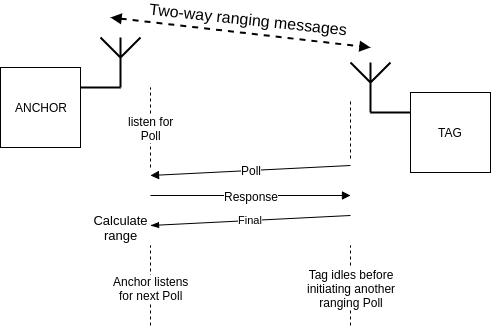
\includegraphics[width=\linewidth]{ranging.png}
    \end{column}
  \end{columns}
\end{frame}

\begin{frame}{Two-way Ranging}
  \begin{columns}[T]
    \begin{column}{0.5\textwidth}
      il \alert{tag} salva RMARKER di
      \begin{itemize}
      \item[-] invio Poll ($Rm_{ps}$)
      \item[-] ricezione Risposta ($Rm_{rr}$)
      \item[-] invio Final ($Rm_{fs}$) (delayed transmission)
      \end{itemize}
    \end{column}
    \begin{column}{0.5\textwidth}
      l' \alert{ancora} salva RMARKER di
      \begin{itemize}
      \item[-] ricezione Poll ($Rm_{pr}$)
      \item[-] spedizione Risposta ($Rm_{rs}$)
      \item[-] ricezione Final ($Rm_{fr}$)
      \end{itemize}
    \end{column}
  \end{columns}
  \begin{center}
    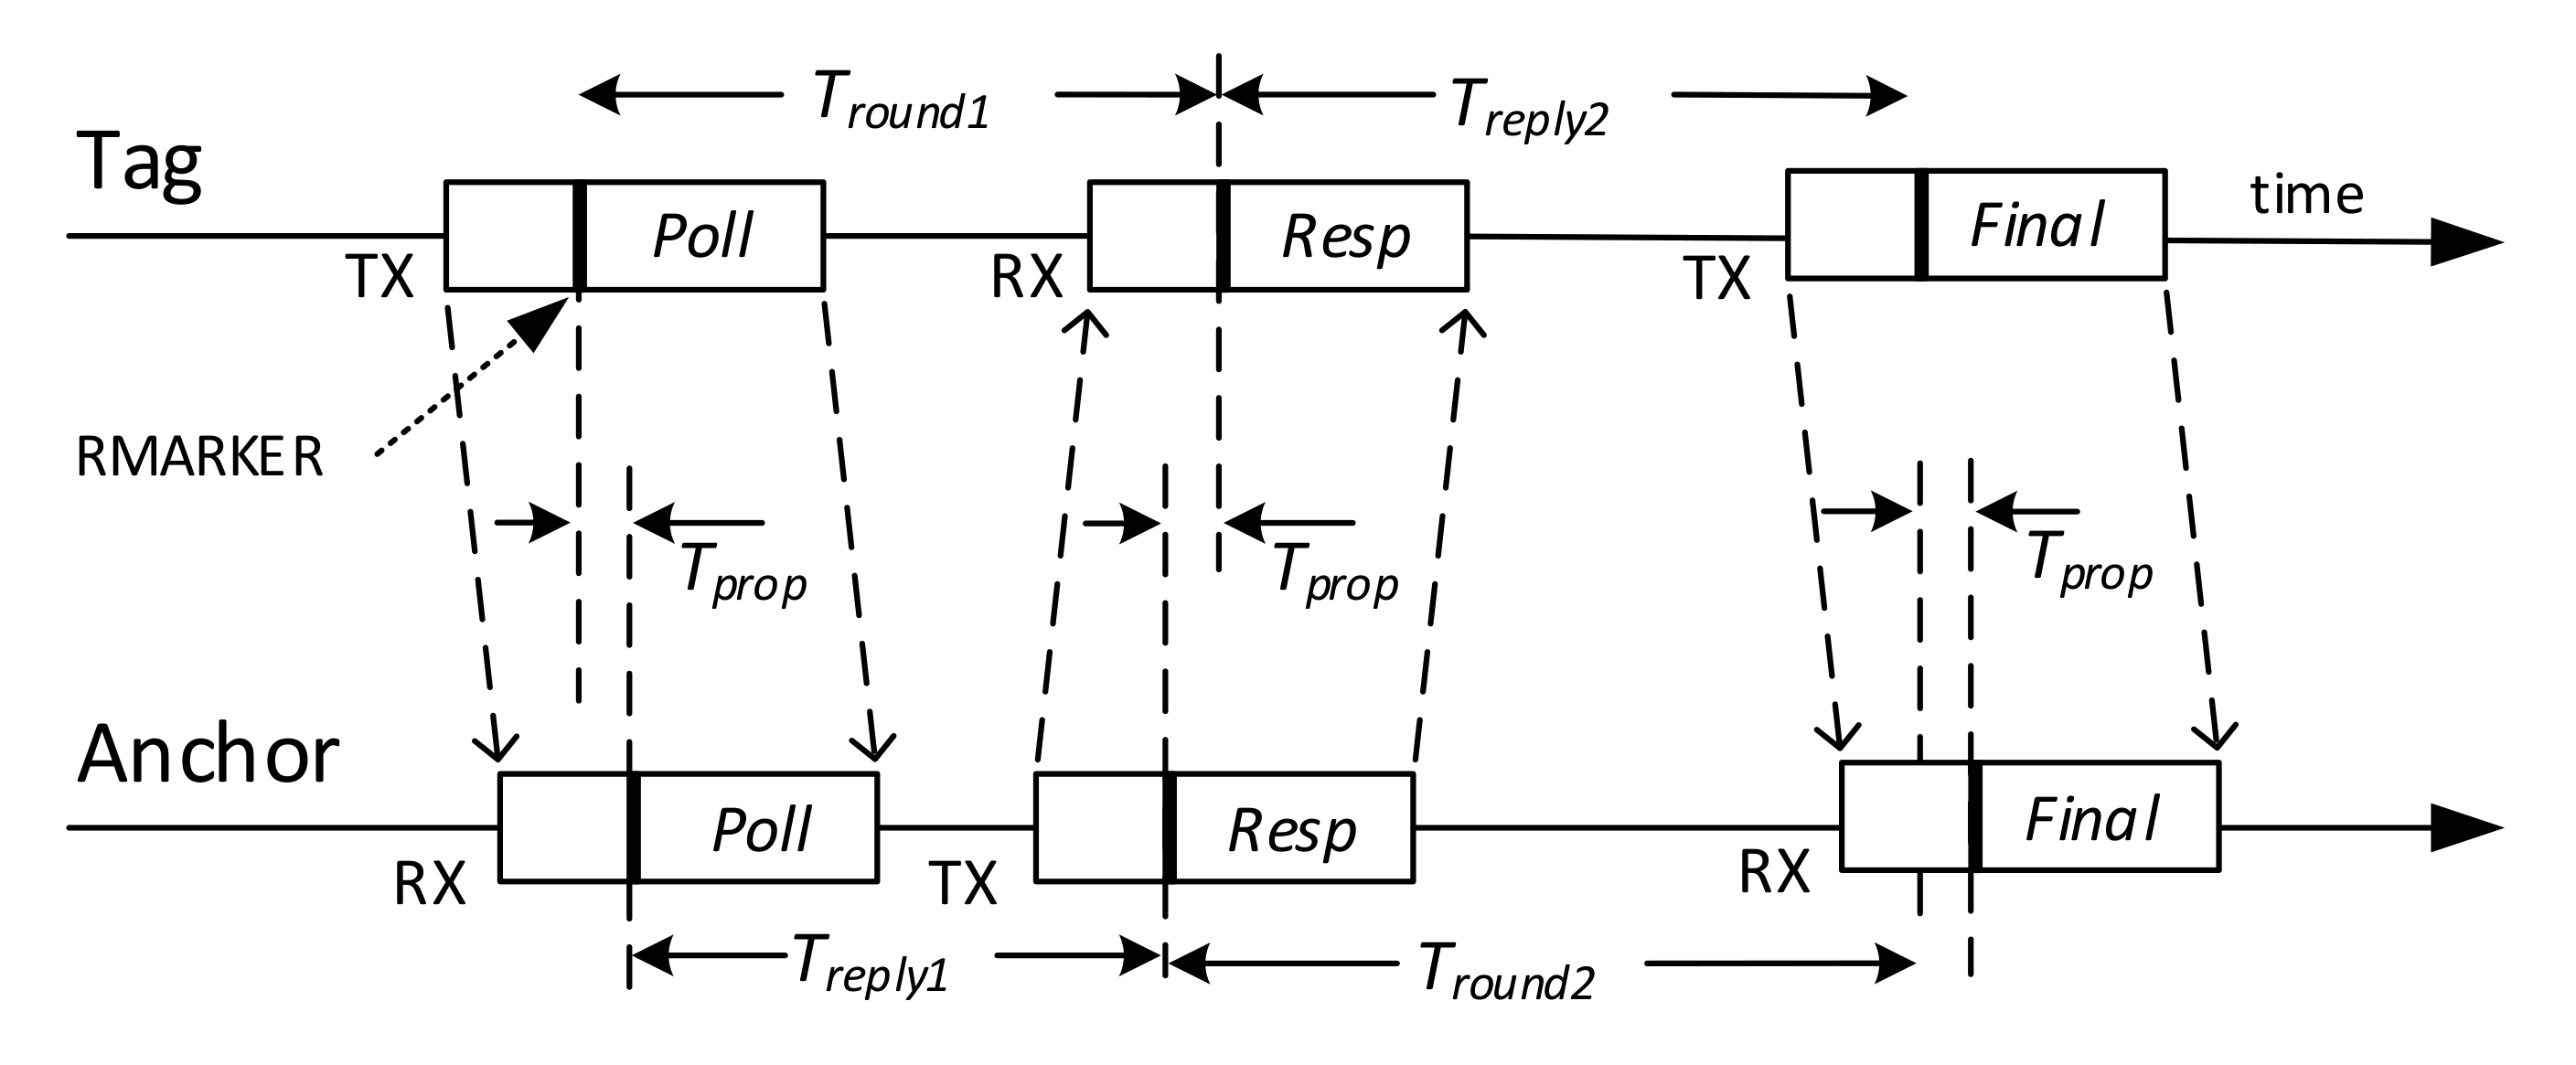
\includegraphics[scale = 0.7]{ranging_with_timings.png}
  \end{center}
  Il tag invia $Rm_{ps}$, $Rm_{rr}$ e $Rm_{fs}$ all'ancora nel Final
\end{frame}

\begin{frame}{Calcolo del ToF}
  Le seguenti quantità sono \alert{calcolate} dall' \alert{ancora} utilizzando i dati raccolti e
  ricevuti dal tag durante un'istanza di ranging
  \[
  \begin{split}
    T_{round1} = Rm_{rr} - Rm_{ps} \quad \quad T_{round2} = Rm_{fs} - Rm_{rr}\\
    T_{reply1} = Rm_{rs} - Rm_{pr} \quad \quad T_{reply2} = Rm_{fr} - Rm_{rs}
  \end{split}
  \]

  Alla ricezione del Final l'ancora calcola il nuovo Tof ($T_{prop}$) che viene inviato al tag nella Risposta al Poll dell'istanza di ranging \alert{successiva}
  \[
  T_{prop} = \frac{T_{round1} T_{round2} - T_{reply1} T_{reply2}}{T_{round1} + T_{round2} + T_{reply1} + T_{reply2}}
  \]
\end{frame}

\begin{frame}{Delayed transmission}
  \begin{alertblock}{Attenzione}
    La necessità di spedire nel messaggio di Final il tempo di spedizione del medesimo richiede
    l'utilizzo della funzione di \emph{delayed transmission} del DW1000.
  \end{alertblock}
  Il tempo di spedizione viene scelto a priori come
  \[
  Rm_{fs} = Rm_{ps} + \Delta
  \]
  dove $\Delta$ è maggiore del tempo impiegato da tutte le ancore per rispondere al tag (attenzione ad aumento di ancore).
  La funzione \emph{delayed transmission} garantisce che l'RMARKER di spedizione del Final coincida con
  $Rm_{fs}$
\end{frame}

\begin{frame}{Frame \& Superframe}
  Il sistema supporta \alert{nativamente} fino 8 tag e 3/4 ancore
  \centering
  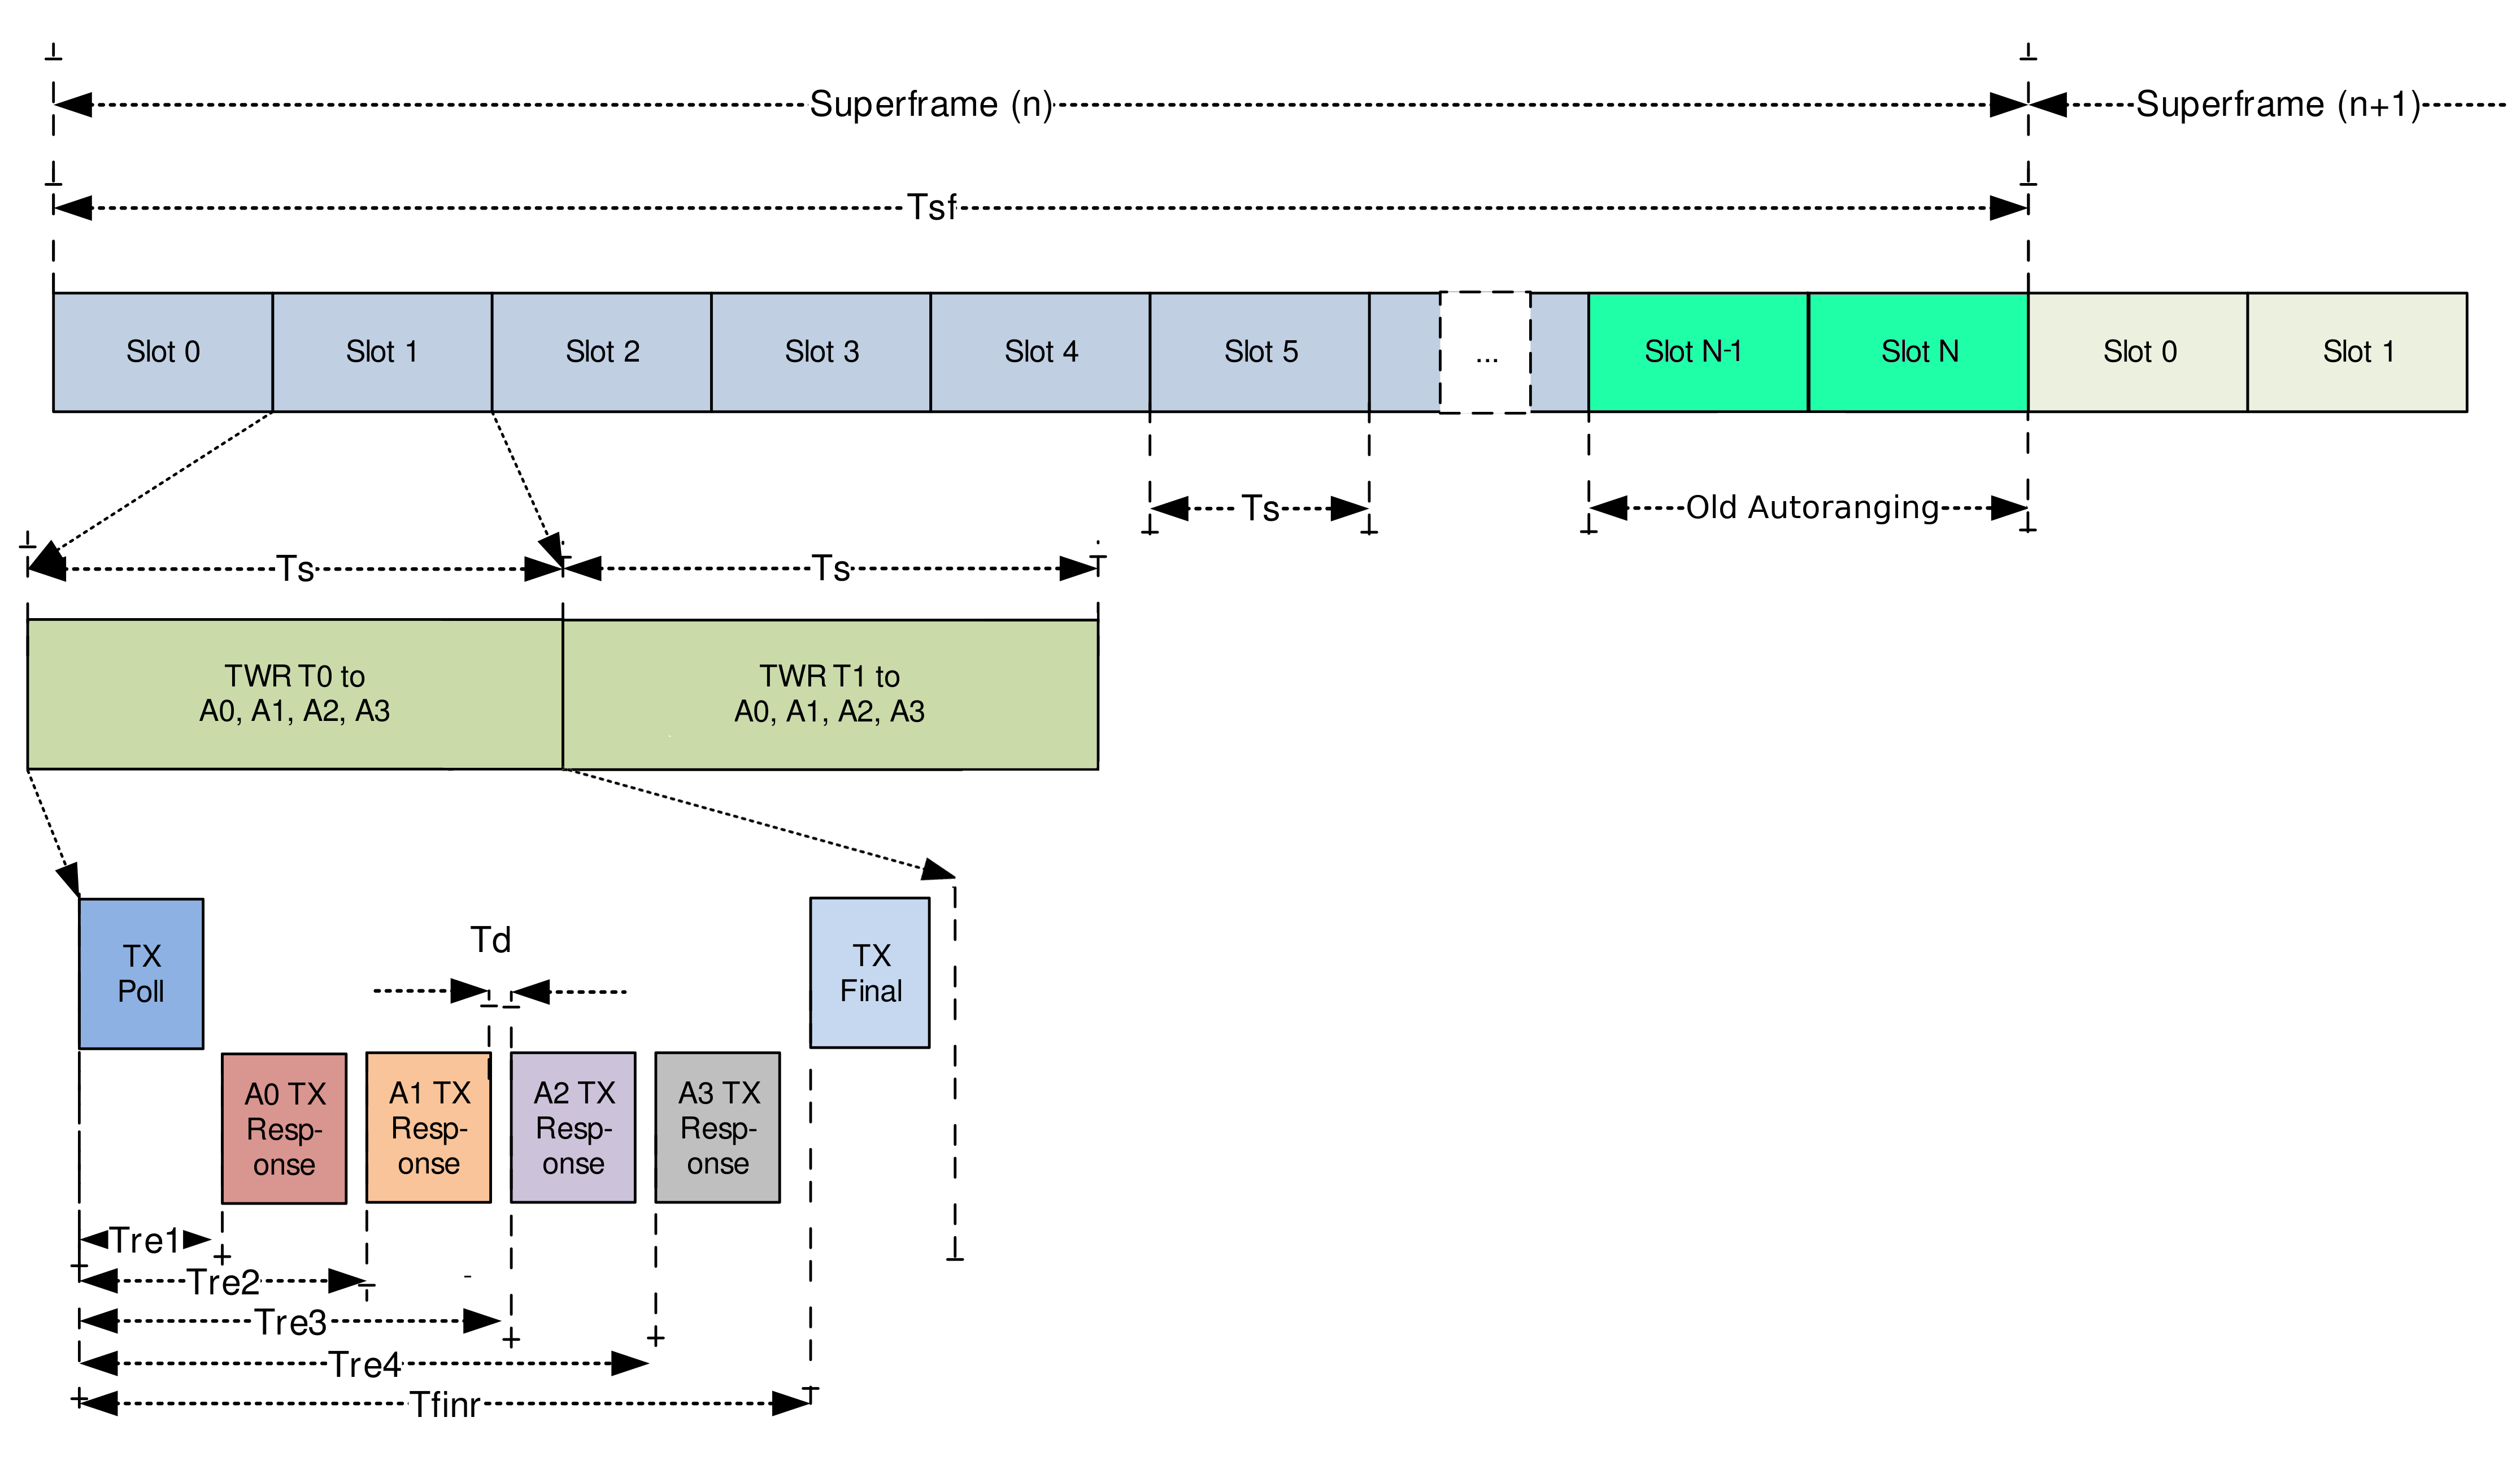
\includegraphics[width=\linewidth]{frame_superframe_a2a.png}
\end{frame}

\begin{frame}{Gestione di più tag}
  Ogni tag invia un messaggio di Poll ogni \alert{activation time} $a_t$
  \[
  a_t = T_{sf} + T_{sr} + T_{sc}
  \]
  \begin{itemize}
  \item[-] $T_{sf}$: durata del Superframe 
  \item[-] $T_{sr}$: alla prima iterazione vale $\SI{10}{\milli\second}$ successivamente vale  $\SI{0}{\milli\second}$
  \item[-] $T_{sc}$: correzione calcolata dall'\alert{Ancora 0} ed inviata al \alert{tag i-esimo} 
  \end{itemize}
\end{frame}

\begin{frame}{Calcolo della correzione $T_{sc}$}
  La correzione viene calcolata in base ad un errore calcolato come la differenza tra il tempo atteso
  d'arrivo del Poll e quello effettivo (dal punto di vista dell'ancora 0)
  \[
  e = t_{i}^{a} - t_{rx}
  \]
  La correzione vale
  \[
  \begin{cases}
    T_{sc} = e \quad \quad \quad \quad \text{se } e < -\frac{T_{sf}}{2}\\
    T_{sc} = T_{sf} + e \quad \quad \text{altrimenti}
  \end{cases}
  \]
\end{frame}

\begin{frame}{Calcolo Calcolo del tempo di attivazione $T_{sc} = e$}
  Il tempo di riattivazione del tag $t_{i+1}^{t}$ è:
  \[
  t_{i+1}^{t} = t_{i}^{t} + T_{sf} + T_{sc} = t_i^a - (\cancel{e} + Tof) + T_{sf} + \cancel{e} = t_i^a - Tof + T_{sf} 
  \]
  \begin{center}
    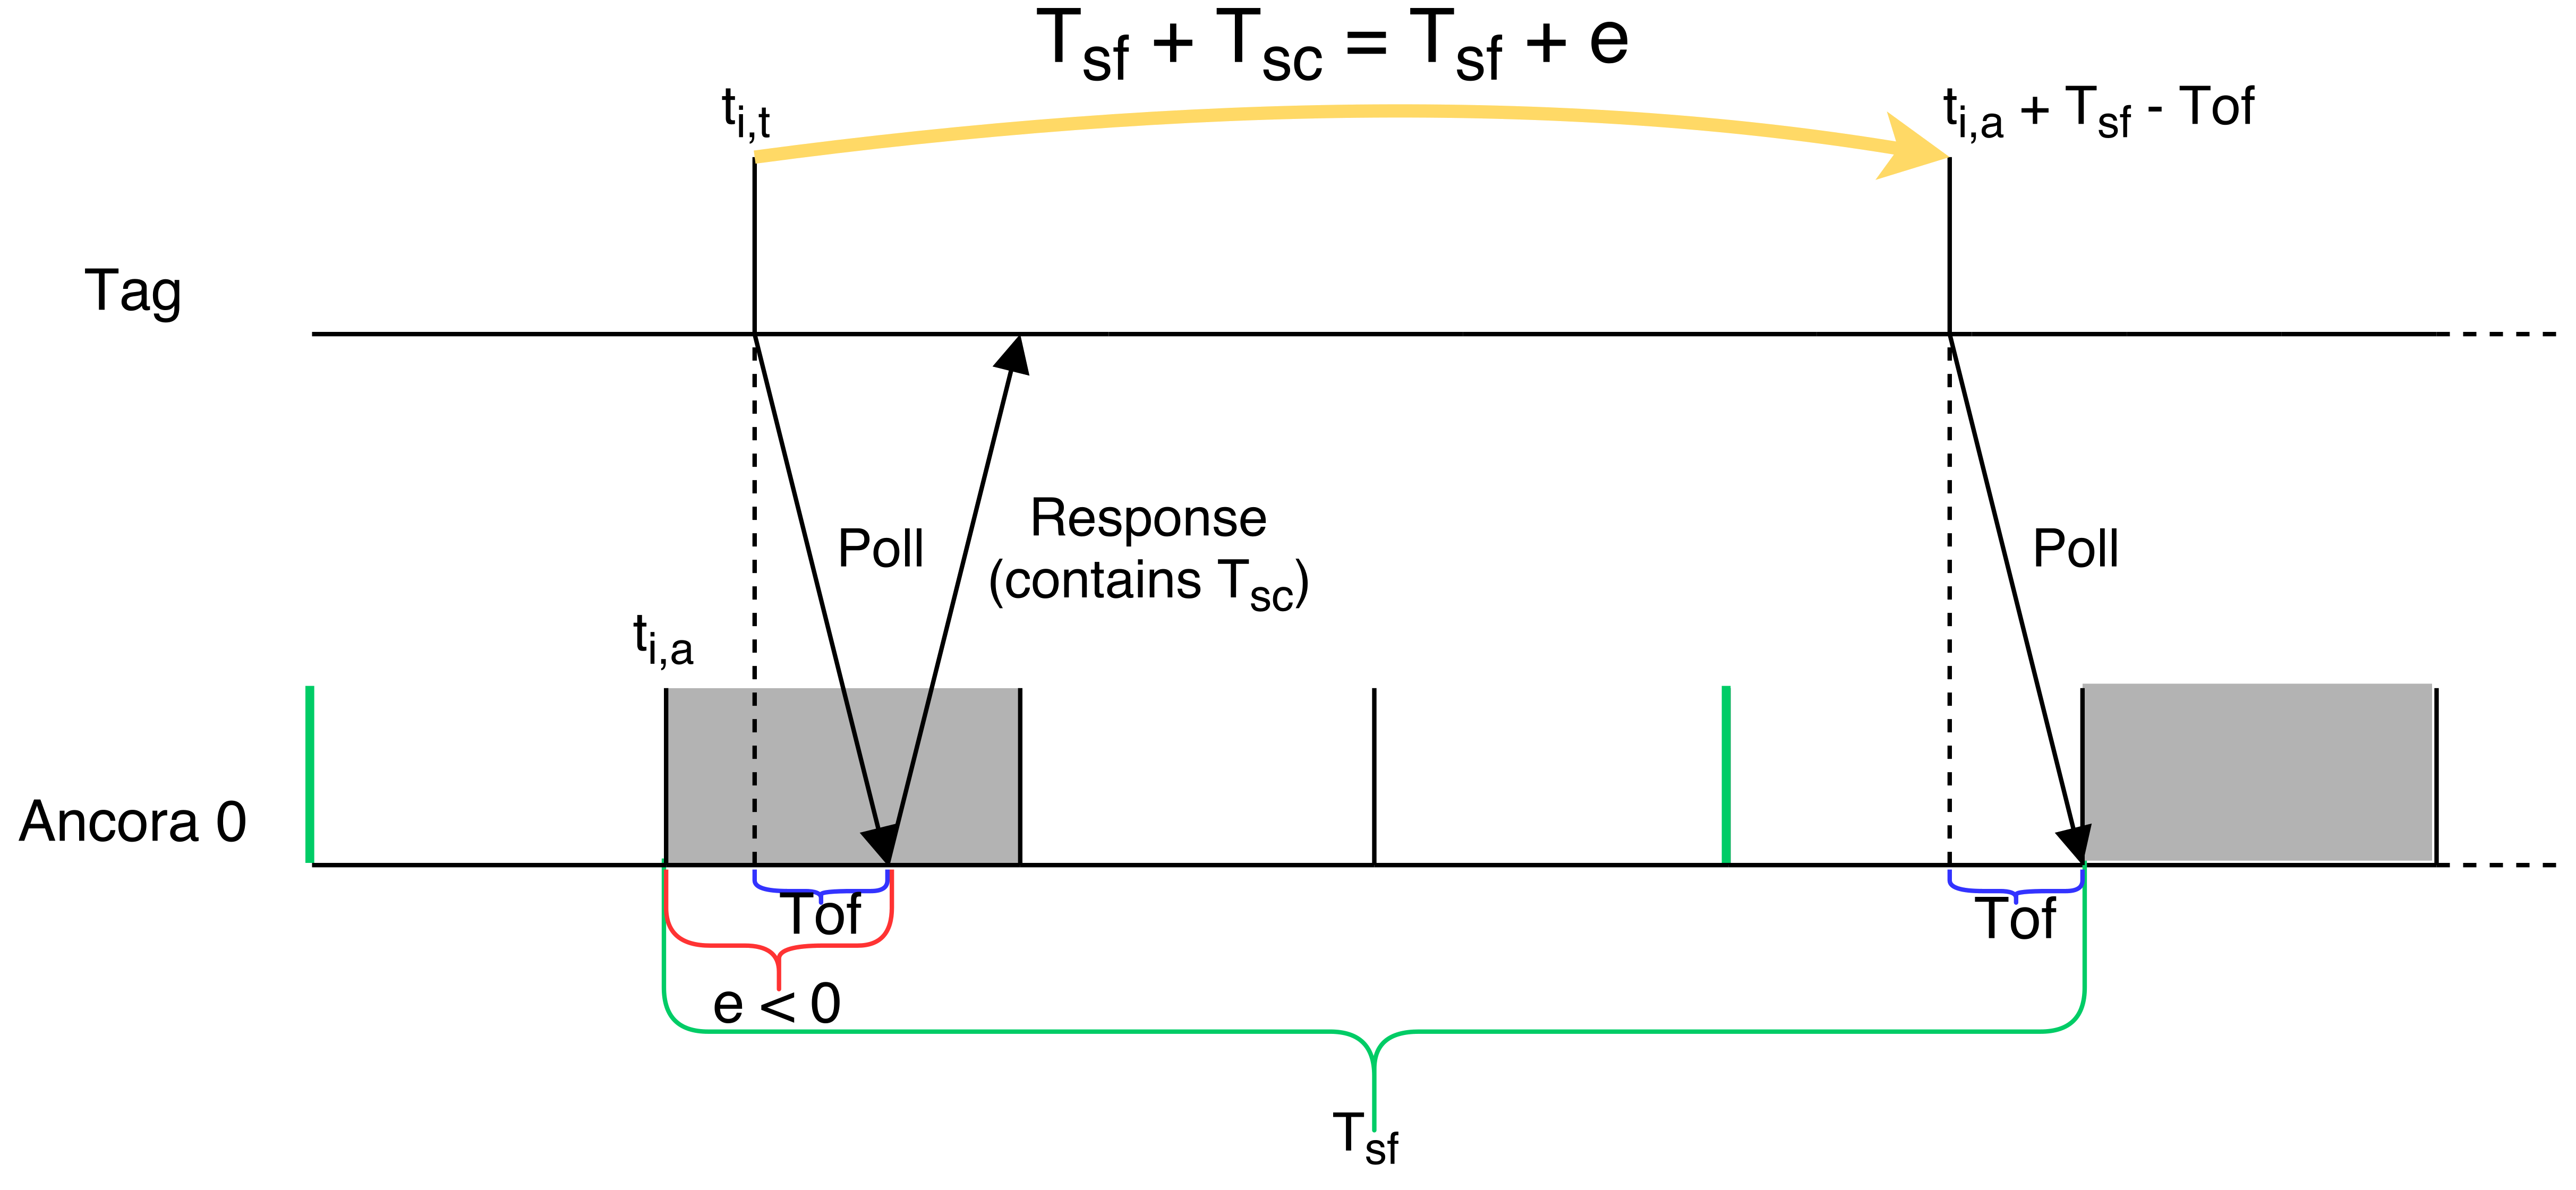
\includegraphics[width=\linewidth]{sleep_correction_less_half_superframe.png}
  \end{center}
\end{frame}

\begin{frame}{Calcolo del tempo di attivazione $T_{sc} = e + T_{sf}$}
  Il tempo di riattivazione del tag $t_{i+1}^{t}$ è:
  \[
  t_{i+1}^{t} = t_{i}^{t} + T_{sf} + T_{sc} = t_i^a - (\cancel{e} + Tof) + T_{sf} + (\cancel{e} + T_{sf}) = t_i^a - Tof + 2T_{sf} 
  \]
  \begin{center}
    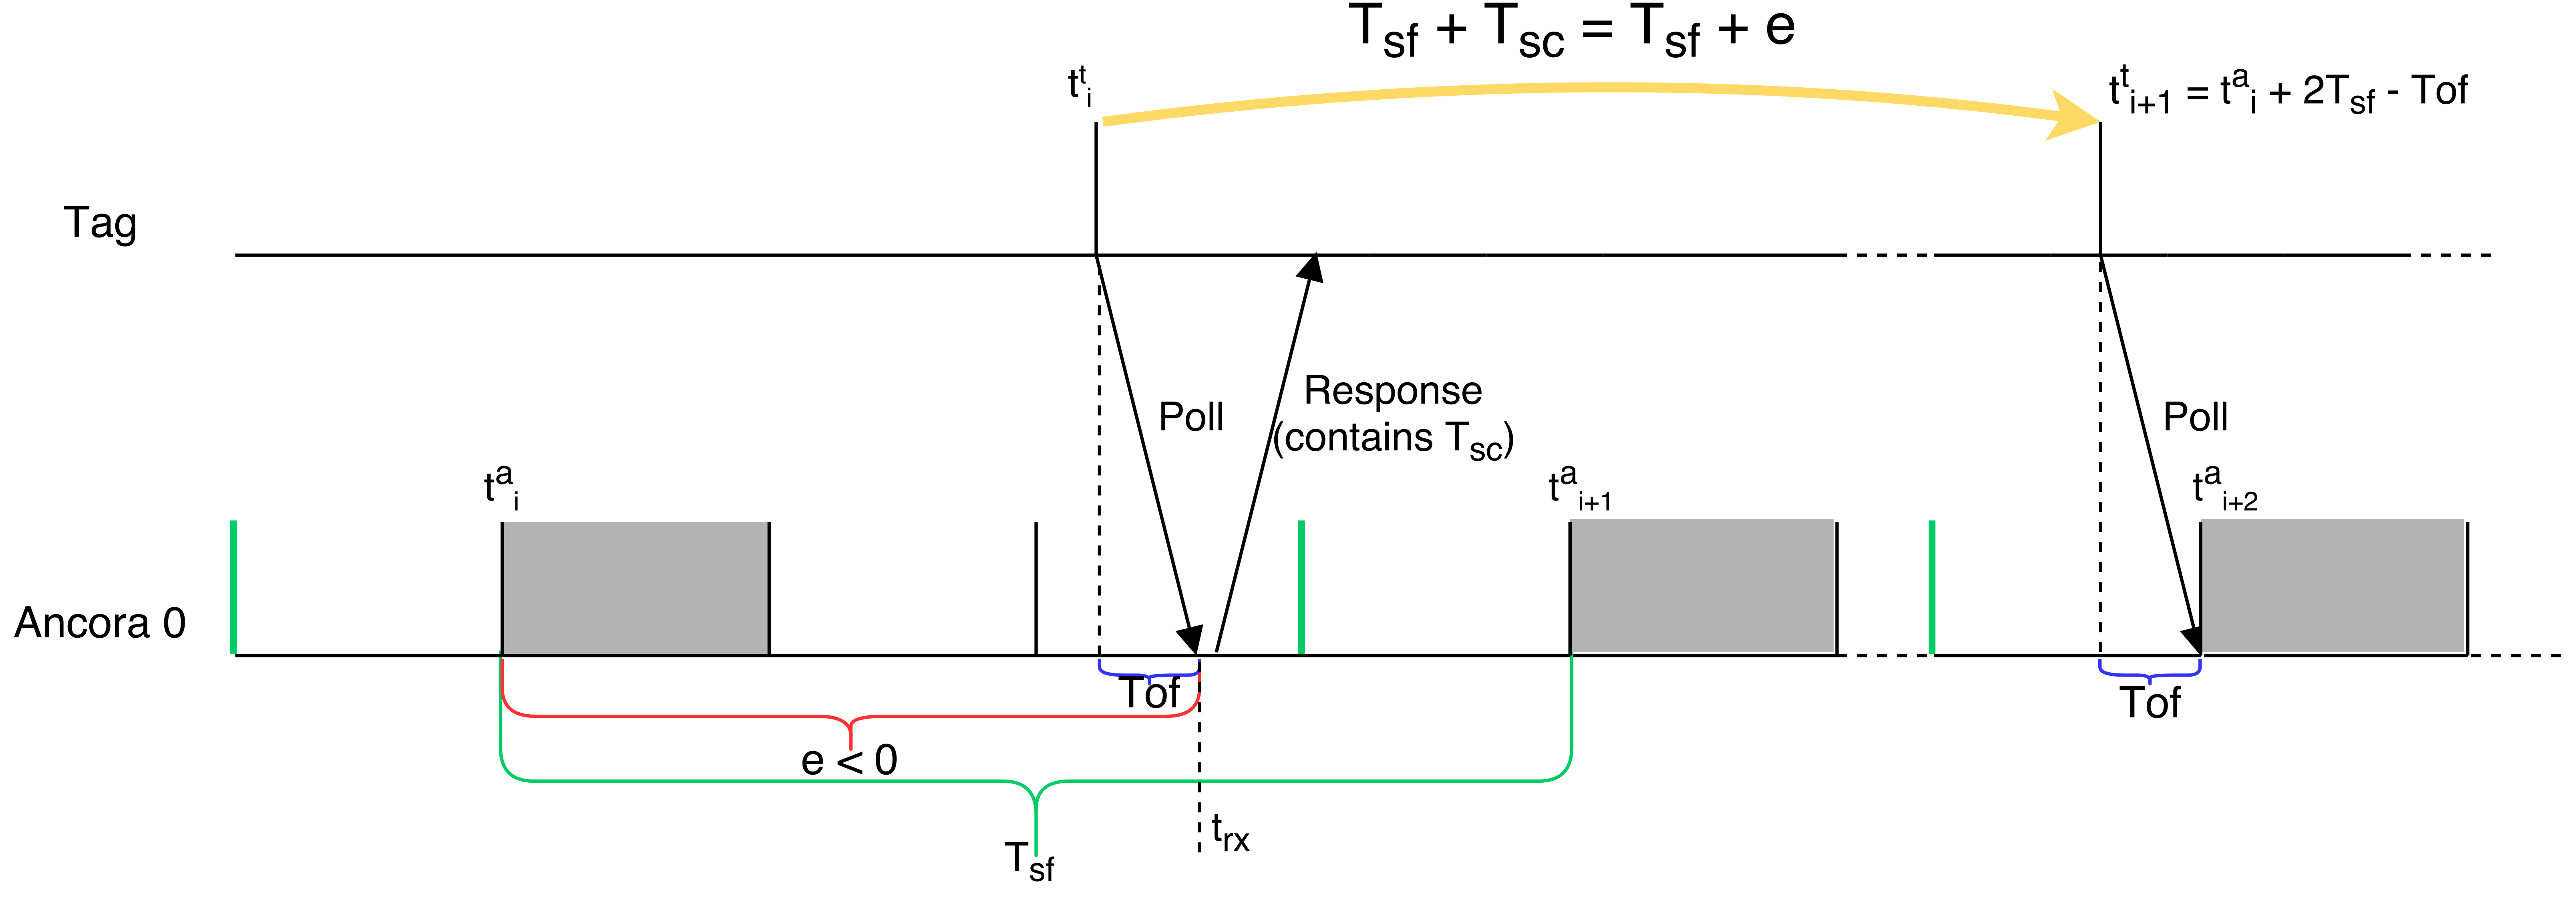
\includegraphics[width=\linewidth]{sleep_correction_greater_half_superframe.png}
  \end{center}
\end{frame}

\begin{frame}{Aumento della frequenza di ranging}
  \begin{center}
    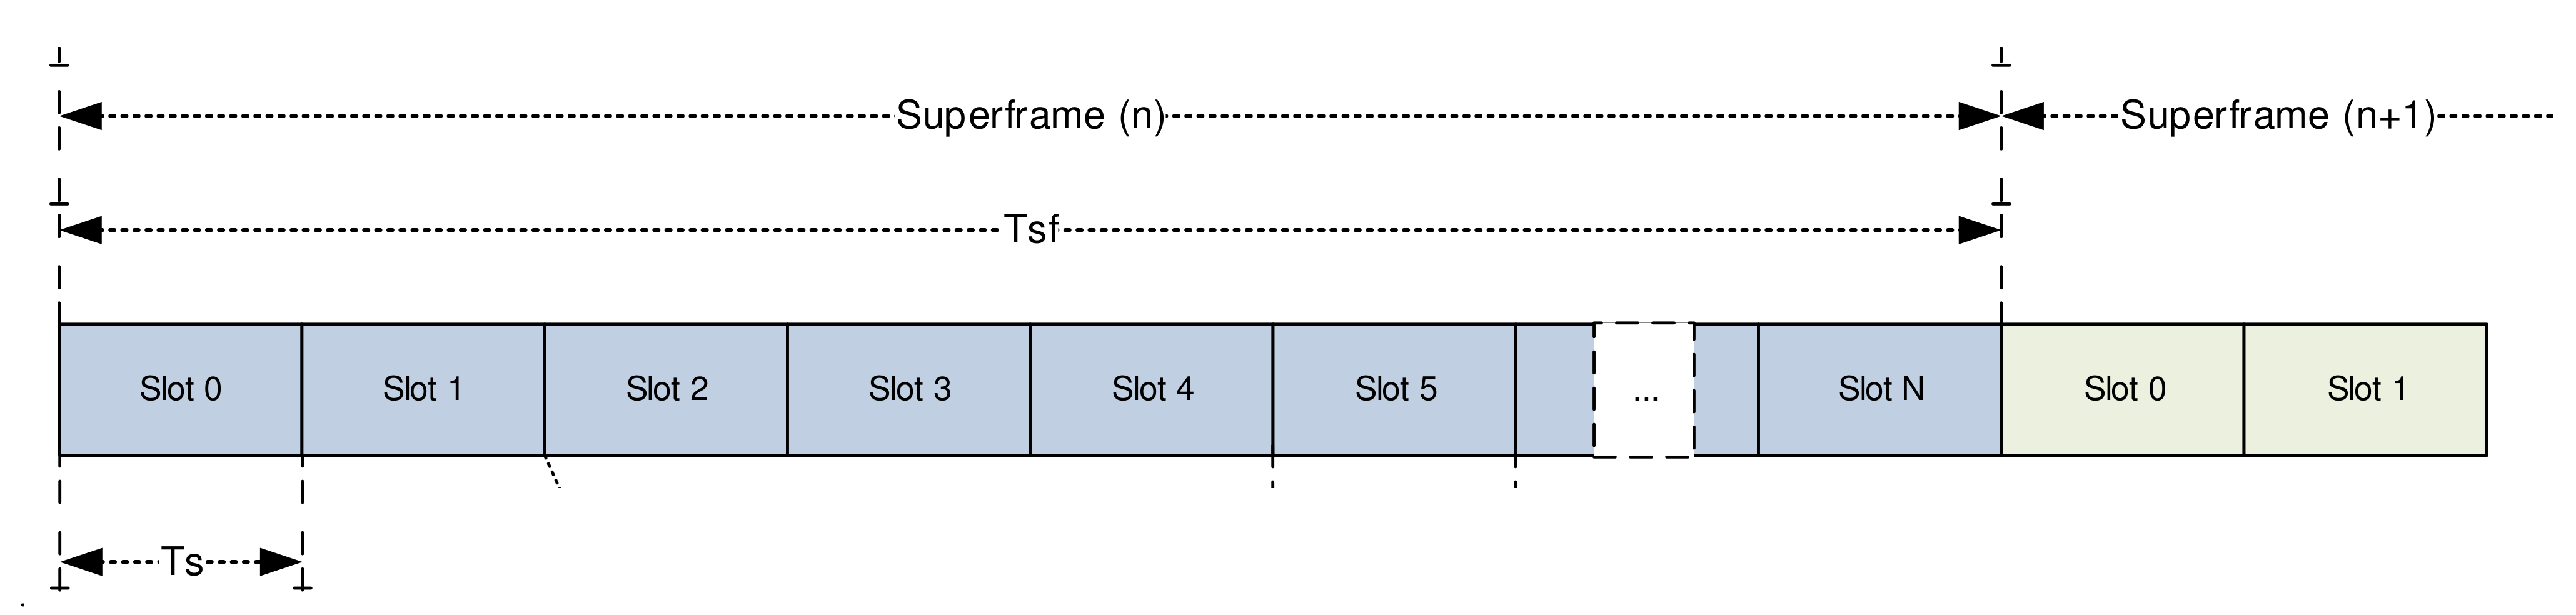
\includegraphics[width=\linewidth]{pmg_frames_removal.png}
  \end{center}
      
  \begin{itemize}
  \item[-] contributo di Pinna, Malagoli, Giannini;
  \item[-] utilizzabile con un solo tag;
  \item[-] $T_{sf} = T_s = \SI{10}{\milli\second}$;
  \item[-] frequenza $ f = \SI{100}{\hertz}$.
  \end{itemize}
\end{frame}
